
\documentclass[10.5pt,a4paper,oneside]{article}
\usepackage[a4paper,left=19mm,right=19mm,top=20mm,bottom=20mm,headheight=21pt]{geometry}
\usepackage{fontspec}
\setmainfont{Linux Libertine O}
\setsansfont{Lato}
\usepackage[english]{babel}
\usepackage{microtype}
\usepackage[dvipsnames,table]{xcolor}
\usepackage{graphicx}
\usepackage{booktabs,tabularx,longtable,array,multirow}
\usepackage{tikz}
\usetikzlibrary{arrows.meta,positioning,fit,calc,shapes.geometric}
\usepackage{fancyhdr,enumitem,titlesec,needspace,tcolorbox,hyperref,amsmath,amssymb}
\usepackage{lastpage,float}
\definecolor{main}{HTML}{184C3E}
\definecolor{deep}{HTML}{12372F}
\definecolor{light}{HTML}{EAF1EC}
\definecolor{warm}{HTML}{F8F7F3}
\definecolor{gold}{HTML}{A47B42}
\definecolor{graytext}{HTML}{5C6864}
\definecolor{line}{HTML}{CED8D2}
\definecolor{alert}{HTML}{8F3A36}
\hypersetup{colorlinks=true,linkcolor=main, urlcolor=main, citecolor=main, pdftitle={Sales AI Management - Unified Enterprise Architecture and 12-Step Implementation Plan},pdfauthor={Sales AI Management - Architecture Reference},pdfsubject={One complete release, secure multi-tenant sales AI platform}}
\pagestyle{fancy}
\fancyhf{}
\fancyhead[L]{\sffamily\small\color{main} SALES AI MANAGEMENT}
\fancyhead[R]{\sffamily\scriptsize\color{graytext} UNIFIED ARCHITECTURE / 2026}
\fancyfoot[L]{\sffamily\scriptsize\color{graytext} Target design - not an implementation audit}
\fancyfoot[R]{\sffamily\scriptsize\color{graytext}\thepage\ / \pageref{LastPage}}
\renewcommand{\headrulewidth}{0.4pt}
\renewcommand{\headrule}{\hbox to\headwidth{\color{line}\leaders\hrule height \headrulewidth\hfill}}
\setlength{\parindent}{0pt}
\setlength{\parskip}{5.5pt}
\setlist[itemize]{leftmargin=5.0mm,itemsep=2pt,topsep=3pt}
\setlist[enumerate]{leftmargin=6mm,itemsep=2pt,topsep=3pt}
\renewcommand{\arraystretch}{1.21}
\titleformat{\section}{\Large\sffamily\bfseries\color{main}}{\thesection.}{0.6em}{}
\titleformat{\subsection}{\large\sffamily\bfseries\color{deep}}{\thesubsection}{0.6em}{}
\titleformat{\subsubsection}{\normalsize\sffamily\bfseries\color{deep}}{\thesubsubsection}{0.6em}{}
\titlespacing*{\section}{0pt}{15pt}{7pt}
\titlespacing*{\subsection}{0pt}{12pt}{5pt}
\newcolumntype{Y}{>{\raggedright\arraybackslash}X}
\newcolumntype{L}[1]{>{\raggedright\arraybackslash}p{#1}}
\newtcolorbox{keybox}[1][]{colback=light,colframe=line,boxrule=.55pt,arc=2pt,left=9pt,right=9pt,top=7pt,bottom=7pt,#1}
\newtcolorbox{riskbox}[1][]{colback=warm,colframe=gold,boxrule=.65pt,arc=2pt,left=9pt,right=9pt,top=7pt,bottom=7pt,#1}
\newcommand{\eyebrow}[1]{{\sffamily\footnotesize\bfseries\color{gold}\MakeUppercase{#1}}}
\newcommand{\tinyhint}[1]{{\sffamily\footnotesize\color{graytext}#1}}
\newcommand{\tblhead}[1]{{\sffamily\bfseries\color{white}#1}}
\newcommand{\cellstrong}[1]{{\sffamily\bfseries\color{deep}#1}}
\AtBeginDocument{\color{black!88}}
\begin{document}
\begin{titlepage}
\thispagestyle{empty}
\begin{tikzpicture}[remember picture,overlay]
\fill[deep] (current page.north west) rectangle ([yshift=-86mm]current page.north east);
\fill[main] ([yshift=-86mm]current page.north west) rectangle ([yshift=-88mm]current page.north east);
\fill[gold] ([xshift=17mm,yshift=-36mm]current page.north west) rectangle ([xshift=68mm,yshift=-37.2mm]current page.north west);
\end{tikzpicture}
\vspace*{21mm}
{\sffamily\large\bfseries\color{white} SYSTEM ARCHITECTURE + EXECUTION BLUEPRINT}\par\vspace{14mm}
{\sffamily\fontsize{30}{36}\selectfont\bfseries\color{white} SALES AI\\[4pt] MANAGEMENT}\par\vspace{8mm}
{\sffamily\Large\color{white!84} Unified Enterprise Architecture}\par
\vspace*{34mm}
\begin{keybox}
\textbf{One product. One complete release. Twelve gated implementation steps.}\\
Multi-tenant B2B/B2C SaaS, CRM, commerce, inventory, procurement, logistics, customer and manager voice AI, 18 logical AI roles, deterministic workflows, analytics, security and operational assurance.
\end{keybox}
\vspace{8mm}
\begin{tabularx}{\textwidth}{@{}L{41mm}Y@{}}
\textbf{Document purpose} & Comprehensive technical target + sequenced implementation and acceptance plan\\
\textbf{Architecture status} & Proposed design; implementation, benchmarks, and security verification are pending\\
\textbf{Security baseline} & 70-security.xlsx (originally STOKORA), with 70 controls + 12 proposed Sales AI extensions\\
\textbf{Delivery process} & Six sprints / two sequential steps per sprint; inspect, implement, test, fix, document, validate\\
\textbf{Prepared} & 17 November 2026\\
\end{tabularx}
\vfill
\tinyhint{LaTeX source included separately for reproducible editing and compilation. The solution is one target system; internal steps are implementation gates, not product versions.}
\end{titlepage}
\tableofcontents
\clearpage

\section{Executive architecture decisions}
\begin{keybox}
\textbf{Target:} a single enterprise Sales AI Management SaaS product with all previously agreed modules and both voice modes. There is no separate V1/V2/V3/V4/V5 product-release scope. The twelve steps below are internal construction and validation checkpoints.
\end{keybox}
\begin{tabularx}{\textwidth}{@{}L{40mm}Y@{}}
\toprule\rowcolor{light}\textbf{Decision} & \textbf{Architecture rule}\\\midrule
Commercial authority & Domain services calculate prices, reserve stock, issue documents, validate payments, authorize transitions and commit state; models only request typed actions.\\
State of record & PostgreSQL is authoritative. Redis is ephemeral/rebuildable, never a second order, payment or stock ledger.\\
AI execution & Direct-read, bounded-reasoning and durable-workflow paths; select the lightest safe path for each intent.\\
Conversation ownership & One active Conversation Supervisor per conversation version, with human handoff suppressing autonomous messages.\\
Agents & 18 logical roles are a capability catalog, not 18 simultaneously running agents or 18 independently deployed services.\\
Voice & Customer Voice Agent and Manager Voice Copilot reuse the same policy and business core; manager permissions are separate.\\
Asynchronous correctness & PostgreSQL transaction + outbox + durable workflows + idempotent consumers + reconciliation.\\
Security & Zero-trust tenant/resource authorization, evidence-based release gating, original 70 controls reclassified for Sales AI, plus 12 AI/voice extensions.\\
Deployment & Modular backend and independently scalable channel, agent, voice, job and inference workloads; evolve topology based on measured load.\\
\bottomrule
\end{tabularx}

\section{Actors, channels and functional scope}
\subsection{Actors and core experiences}
\begin{tabularx}{\textwidth}{@{}L{33mm}Y@{}}
\toprule\rowcolor{light}\textbf{Actor} & \textbf{Capability boundary}\\\midrule
Customer & Product questions, verified quotes, own order/payment/ETA status, bookings, support, returns, optional voice and chat.\\
Sales representative & Assigned leads, opportunities, conversations, customer briefs, proposals, tasks and safe copilot assistance.\\
Support / operations & Human handoff, tickets, procurement, warehouse movements, fulfilment and assigned service actions.\\
Manager / owner & Role-scoped dashboards, exact-term approvals, policy configuration, alerts, reports, privileged voice copilot.\\
Tenant administrator & Users/roles, channels, usage, security settings, feature flags and integrations for their tenant only.\\
Platform administrator & Service health, billing/tenancy infrastructure, incident response and support-access controls with explicit audit.\\
\bottomrule
\end{tabularx}
\subsection{Functional business domains}
\small
\begin{longtable}{@{}L{33mm}L{58mm}L{66mm}@{}}
\toprule\rowcolor{light}\textbf{Domain} & \textbf{Responsibilities} & \textbf{Owned invariants / outputs}\\\midrule
\endfirsthead
\toprule\rowcolor{light}\textbf{Domain} & \textbf{Responsibilities} & \textbf{Owned invariants / outputs}\\\midrule
\endhead
SaaS and IAM & Tenant, site, member, role, subscription, quotas, feature controls & Authenticated membership, resource policy and tenant context\\
Omnichannel & Web/app, WhatsApp, email/Gmail, telephony, unified inbox & Verified provider, durable ingest, dedupe, ownership and consent\\
CRM and pipeline & Leads, contacts, B2B accounts, opportunity stages, assignments & Provenance, controlled identity linking, SLA routing\\
Catalog and pricing & SKU/variants, catalogs, taxes, currencies, margins & Price-list versions, minor-unit arithmetic, tax rules\\
Quotations & Quote drafts, pro-forma, discounts and approval requests & Exact-term version/hash, expiry, revaluation on accept\\
Orders and payments & Sales orders, online/bank/COD payments, invoices, reconciliation & Idempotent order commit, signed payment evidence, no AI-paid inference\\
Inventory and procurement & Multi-warehouse movements, holds, backorder, RFQ, PO, receipts & Append-only movements, capacity checks, approved purchasing\\
Fulfilment & Pick/pack, carriers, shipping status, proof of delivery & No state regression from out-of-order carrier events\\
Customer service & Tickets, returns, warranty, refund requests, escalations & Explicit lifecycle, inspected restock, provider-confirmed refund\\
Scheduling & Sales demonstrations, appointments, callbacks & Current availability and atomic booking confirmation\\
Documents & Quotes, invoices, contracts, shipment and support artifacts & Approved template, immutable issued bytes and checksum\\
Analytics & Pipeline, revenue, team, margins, forecasts, KPI reports & Versioned KPI definitions, report watermark and scoped read models\\
Campaigns & Follow-ups, outreach proposals, notifications and reminders & Consent, frequency caps, quiet hours, delivery-side rechecks\\
\bottomrule
\end{longtable}
\normalsize

\section{Logical system architecture}
\begin{figure}[H]
\centering
\resizebox{\textwidth}{!}{%
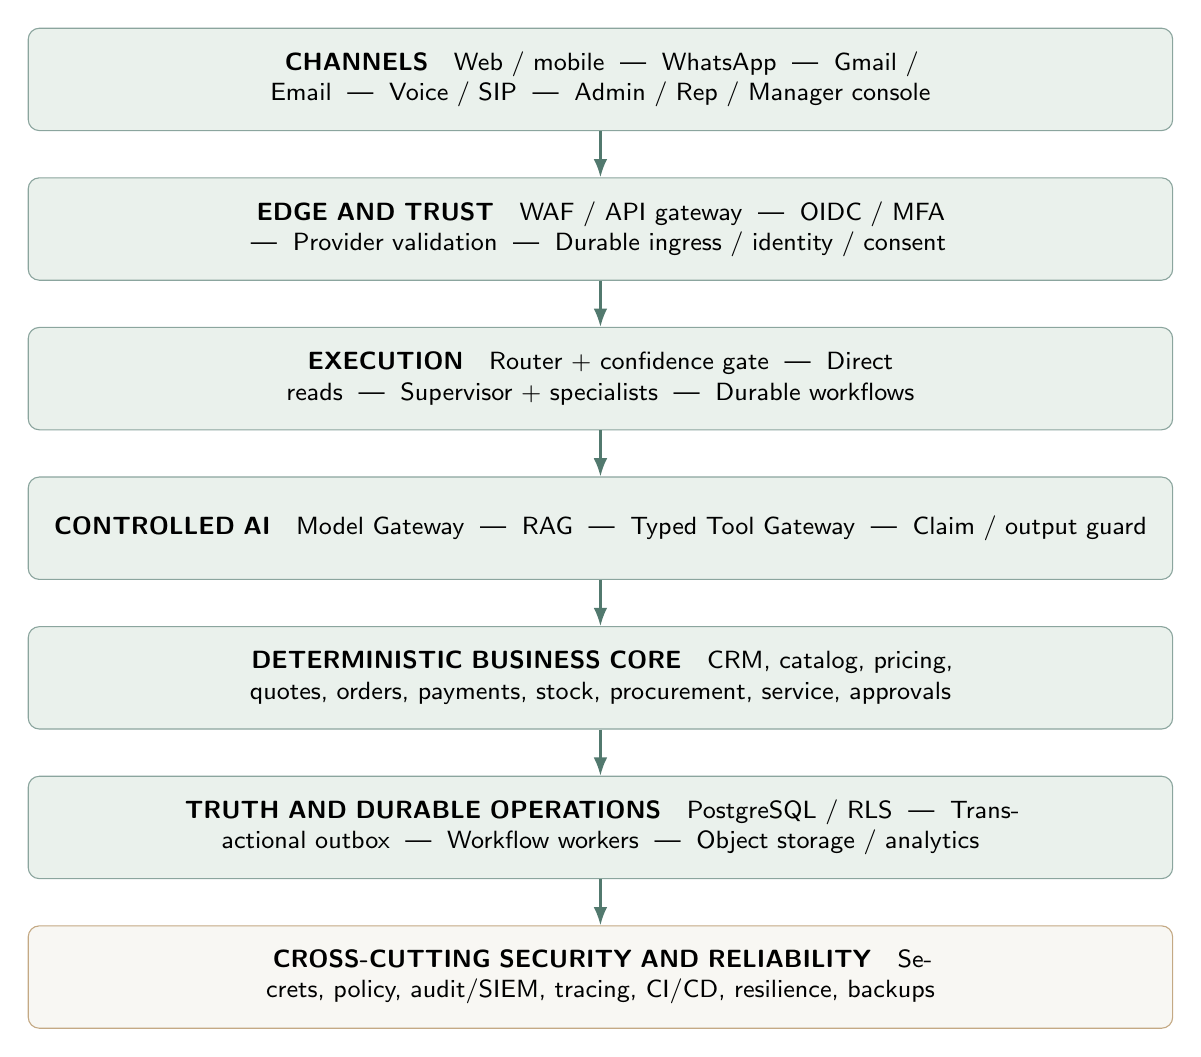
\begin{tikzpicture}[>=Latex, every node/.style={font=\sffamily\small}, layer/.style={draw=main!50,rounded corners=4pt,fill=light,minimum height=13mm,text width=143mm,align=center}, edge/.style={-Latex,thick,draw=main!75}]
\node[layer] (c) at (0,0) {\textbf{CHANNELS}\quad Web / mobile \;|\; WhatsApp \;|\; Gmail / Email \;|\; Voice / SIP \;|\; Admin / Rep / Manager console};
\node[layer] (g) at (0,-1.9) {\textbf{EDGE AND TRUST}\quad WAF / API gateway \;|\; OIDC / MFA \;|\; Provider validation \;|\; Durable ingress / identity / consent};
\node[layer] (e) at (0,-3.8) {\textbf{EXECUTION}\quad Router + confidence gate \;|\; Direct reads \;|\; Supervisor + specialists \;|\; Durable workflows};
\node[layer] (a) at (0,-5.7) {\textbf{CONTROLLED AI}\quad Model Gateway \;|\; RAG \;|\; Typed Tool Gateway \;|\; Claim / output guard};
\node[layer] (b) at (0,-7.6) {\textbf{DETERMINISTIC BUSINESS CORE}\quad CRM, catalog, pricing, quotes, orders, payments, stock, procurement, service, approvals};
\node[layer] (d) at (0,-9.5) {\textbf{TRUTH AND DURABLE OPERATIONS}\quad PostgreSQL / RLS \;|\; Transactional outbox \;|\; Workflow workers \;|\; Object storage / analytics};
\node[layer,fill=warm,draw=gold!65] (s) at (0,-11.4) {\textbf{CROSS-CUTTING SECURITY AND RELIABILITY}\quad Secrets, policy, audit/SIEM, tracing, CI/CD, resilience, backups};
\foreach \x/\y in {c/g,g/e,e/a,a/b,b/d,d/s} \draw[edge] (\x) -- (\y);
\end{tikzpicture}%
}
\caption{Trust-oriented logical architecture. Every cross-layer action is authorized; arrows do not grant unrestricted access.}
\end{figure}
The ingestion gateway authenticates external channel callbacks, stores inbound events \emph{before} batching/debounce, deduplicates provider IDs and normalizes payloads. The routing layer checks stop/consent and human ownership before choosing one of three execution paths. The backend re-authorizes every side effect when it executes.
\subsection{Three execution classes}
\begin{tabularx}{\textwidth}{@{}L{30mm}Y Y@{}}
\toprule\rowcolor{light}\textbf{Path} & \textbf{Use} & \textbf{Guardrails}\\\midrule
Direct & Simple FAQ or current authorized order read & Typed read tool, verified record/version, response template and send check\\
Reasoning & Comparison, multi-domain explanation, quote assistance & One supervisor, bounded delegation, tool allowlists, evidence envelope, output guard\\
Workflow & Approval, payment wait, fulfilment, returns, outbound campaigns & Durable state, timers, idempotency, retries, human approval and reconciliation\\
\bottomrule
\end{tabularx}

\section{AI agents, tools and model architecture}
\begin{keybox}
\textbf{18 logical roles = 1 router + 1 conversation supervisor + 9 interactive specialists + 6 background agents + 1 rep copilot.} Output Guard and offline Quality Reviewer are independent protection/evaluation components, not autonomous commercial agents. Both voice modes use this shared catalog.
\end{keybox}
\small
\begin{longtable}{@{}L{13mm}L{47mm}L{95mm}@{}}
\toprule\rowcolor{light}\textbf{ID} & \textbf{Role} & \textbf{Bounded responsibility}\\\midrule
\endfirsthead\toprule\rowcolor{light}\textbf{ID} & \textbf{Role} & \textbf{Bounded responsibility}\\\midrule\endhead
R00 & Router / confidence gate & Classify intent, language, risk, urgency and execution class; no writes.\\
S00 & Conversation Supervisor & Own a turn, choose specialists, merge evidence, prepare handoff or guarded reply.\\
A01 & Qualification / CRM & Capture stated facts, qualify leads, request scoped CRM commands.\\
A02 & Product / Knowledge & Approved catalog and authorized RAG answers; verify product evidence.\\
A03 & Quote / Pricing & Prepare terms and submit pricing/issue requests; never invent amounts.\\
A04 & Order / Payment & Customer-scoped order, payment and refund requests; verify provider truth.\\
A05 & Scheduling & Find valid slots and request confirmed booking.\\
A06 & Negotiation / Objections & Draft approved commercial alternatives; no unauthorized concessions.\\
A07 & Support / Returns & Ticket, return and warranty assistance with escalation.\\
A08 & Account Management & Governed renewals, reorders and account check-ins.\\
A09 & Documents & Draft structured document requests; issuance owned by service.\\
B01 & Outreach & Draft approved campaigns and follow-up content; notification service controls sends.\\
B02 & Research & Source-backed company/account intelligence; no direct writes.\\
B03 & Pipeline Coach & Propose rep tasks, identify stale deals and SLA risks.\\
B04 & Analyst & Explain governed KPI and forecast read models.\\
B05 & Knowledge Curator & Suggest reviewed/traceable knowledge updates; no direct publishing.\\
B06 & Incident Responder & Diagnose alerts and propose tightly allowlisted reversible runbooks.\\
I01 & Sales Rep Copilot & User-scoped briefs, reply drafts and CRM change proposals.\\
\bottomrule
\end{longtable}\normalsize
\subsection{Agent invariants and model gateway}
Each run has a trusted tenant/actor context, conversation version, request ID, time/latency budget, tool allowlist, prompt/model/tool versions, source references and a structured result envelope. Deny unknown fields, stale versions and cross-tenant references. A model may request but never issue its own privileged authorization token.
\begin{tabularx}{\textwidth}{@{}L{39mm}Y@{}}
\toprule\rowcolor{light}\textbf{Model Gateway duty} & \textbf{Behavior}\\\midrule
Tiered inference & Fast classifier/FAQ path; stronger reasoning for complex work; dedicated low-latency speech path.\\
Replaceable backends & Provider adapters for hosted or local models; no provider-specific permission bypass.\\
Budget and overload & Limits on tokens, delegation, concurrency, cost, timeouts, and per-tenant consumption.\\
Observability & Prompt/model/tool versions, queue wait, p95, fallback causes, token cost, policy outcomes.\\
Evidence and guards & Schema checks, freshness, exact money/status claims, privacy and output policy before sending.\\
\bottomrule
\end{tabularx}

\section{Dual-mode voice architecture}
\begin{figure}[H]
\centering
\resizebox{.97\textwidth}{!}{%
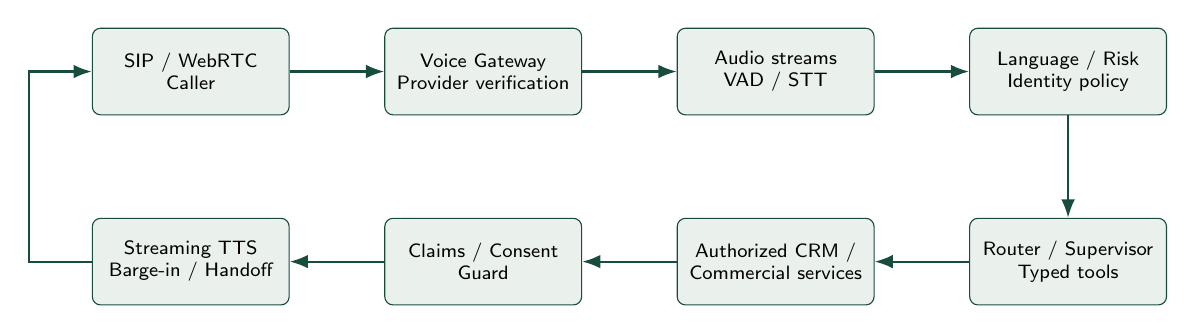
\begin{tikzpicture}[>=Latex,node distance=10mm and 12mm, every node/.style={font=\sffamily\scriptsize},bx/.style={draw=main,rounded corners=3pt,fill=light,minimum width=25mm,minimum height=11mm,align=center}, ar/.style={-Latex,draw=main,thick}]
\node[bx] (call) {SIP / WebRTC\\Caller};
\node[bx,right=of call] (edge) {Voice Gateway\\Provider verification};
\node[bx,right=of edge] (media) {Audio streams\\VAD / STT};
\node[bx,right=of media] (route) {Language / Risk\\Identity policy};
\node[bx,below=13mm of route] (or) {Router / Supervisor\\Typed tools};
\node[bx,left=of or] (core) {Authorized CRM /\\Commercial services};
\node[bx,left=of core] (guard) {Claims / Consent\\Guard};
\node[bx,left=of guard] (tts) {Streaming TTS\\Barge-in / Handoff};
\draw[ar](call)--(edge);\draw[ar](edge)--(media);\draw[ar](media)--(route);\draw[ar](route)--(or);\draw[ar](or)--(core);\draw[ar](core)--(guard);\draw[ar](guard)--(tts);\draw[ar](tts.west) -- ++(-8mm,0) |- (call.west);
\end{tikzpicture}%
}
\caption{Common voice pipeline; caller permissions depend on customer/manager mode and session authentication.}
\end{figure}
\begin{tabularx}{\textwidth}{@{}L{40mm}Y Y@{}}
\toprule\rowcolor{light}\textbf{Function} & \textbf{Customer Voice Agent} & \textbf{Manager Voice Copilot}\\\midrule
Identity & Caller must verify identity before sensitive account/order disclosures & Authenticated employee session; MFA/step-up for consequential requests\\
Read scope & Catalog, own authorized quote/order/support and booking records & Assigned/team/tenant KPI and operational reports according to role\\
Writes & Request quote, case or booking; explicit confirmation and normal domain policy & Can propose action or start approval; voice alone cannot approve/sign/execute high-risk actions\\
Handoff & Transfer to support/rep with scoped context and suppression of AI replies & Transfer to internal authorized operator/approval interface\\
Recordings & Disabled unless lawful/approved policy and notice; controlled retention & Strictly controlled, protected and access logged\\
Languages & Darija, Arabic, French, English, Arabizi and code-switching evaluated separately & Same multilingual testing plus financial/operational vocabulary\\
\bottomrule
\end{tabularx}\par\medskip
Sensitive information must not be disclosed merely because a caller knows a telephone number or uses a convincing synthetic voice. Test replay, spoofing, cross-call memory isolation, prompt injection through audio/transcriptions and telephone/WS abuse. Voice relies on the same domain-authoritative truth and guardrails as text channels.

\section{Transactional business core and workflows}
\subsection{Authoritative business state machines}
\small
\begin{longtable}{@{}L{30mm}L{130mm}@{}}
\toprule\rowcolor{light}\textbf{Aggregate} & \textbf{Allowed lifecycle and invariants}\\\midrule
\endfirsthead\toprule\rowcolor{light}\textbf{Aggregate} & \textbf{Allowed lifecycle and invariants}\\\midrule\endhead
Quote & draft $\rightarrow$ priced $\rightarrow$ approval (when applicable) $\rightarrow$ issued $\rightarrow$ sent $\rightarrow$ accepted / rejected / expired; exact-term hash, price and stock recheck.\\
Approval & pending $\rightarrow$ approved / rejected / changes requested / expired / superseded; one-use and tied to precise object version.\\
Order & created $\rightarrow$ awaiting payment / confirmed $\rightarrow$ picking $\rightarrow$ shipped $\rightarrow$ delivered $\rightarrow$ completed; cancel/refund policy branches.\\
Payment & pending $\rightarrow$ authorized / paid / failed / expired; provider-verified evidence and reconciliation control progression.\\
Reservation & held $\rightarrow$ committed / released / expired; atomic stock capacity, separate backorder state.\\
Return & requested $\rightarrow$ authorized $\rightarrow$ received $\rightarrow$ inspected $\rightarrow$ restocked / rejected $\rightarrow$ refunded.\\
Purchase order & draft $\rightarrow$ approved $\rightarrow$ issued $\rightarrow$ partially received $\rightarrow$ received / closed / cancelled.\\
Document & draft $\rightarrow$ approved $\rightarrow$ issued $\rightarrow$ sent; issued bytes immutable, correction linked.\\
Conversation & agent/human ownership $\rightarrow$ resolved / closed; human ownership silences autonomous response.\\
\bottomrule
\end{longtable}\normalsize
\subsection{End-to-end commercial transaction}
\begin{enumerate}
\item Verify customer and product, currency, quantity/UOM and current catalog and customer entitlements.
\item Price deterministically; calculate tax, margin and discounts with versioned rules.
\item Persist quote draft, exact approval requirements and final issued artifact/version.
\item Accept by an idempotent command; commit order plus reservation/backorder intent atomically.
\item Obtain payment through provider mechanisms; update status only using verified evidence or controlled reconciliation.
\item Fulfil through stock movements, picking/packing, carrier state and proof of delivery.
\item Emit outbox events, notifications and audit records, using committed state as source of truth.
\item Handle cancellations/returns/refunds through guarded state transitions and compensation.
\end{enumerate}
\subsection{Workflow and event contract}
Transactional changes and outbox records are committed together in PostgreSQL. Durable workers handle timers, external callbacks, retry/backoff, dead-letter queues, compensation and provider reconciliation. Use Temporal (or equivalent) as the workflow authority. n8n is only for ancillary integrations; it is not a second transactional engine.
\begin{keybox}
\textbf{Minimum command fields:} request ID, trusted tenant/actor scope, idempotency key, expected aggregate version, typed payload, deadline, authorization result and correlation ID.\\
\textbf{Minimum event fields:} event ID, tenant ID, aggregate type/ID, schema version, occurred-at, correlation/causation IDs, idempotency scope and consumer ordering assumptions.
\end{keybox}

\section{Data architecture and integration contracts}
\begin{tabularx}{\textwidth}{@{}L{32mm}Y@{}}
\toprule\rowcolor{light}\textbf{Storage tier} & \textbf{Recommended responsibility}\\\midrule
PostgreSQL / RLS & Authoritative contacts, messages, quotes, payments, ledgers, approvals, tickets, events; transaction consistency and row restrictions.\\
Redis & Ephemeral cache, short-lived locks with safe fencing, throttling and transient coordination; rebuildable.\\
Object storage & Private quotes, invoices, attachments, approved voice recordings, immutable issued documents; signed access after authorization.\\
pgvector / knowledge & Provenance-indexed documents with tenant/role/document ACL enforcement before retrieval; never cross-tenant by similarity alone.\\
Analytics read models & KPI definitions, snapshot/watermark, read permissions and heavier reporting separated from transactional hot paths.\\
Backup/archive & Encrypted point-in-time recovery, retention, tested restore, independent recovery credentials and logs.\\
\bottomrule
\end{tabularx}
\subsection{Illustrative main table families}
\texttt{tenants, users, memberships, roles, policies, subscriptions, channels, conversations, messages, contacts, companies, leads, opportunities, products, price\_lists, quotes, quote\_items, approvals, orders, order\_items, payments, invoices, warehouses, stock\_movements, stock\_reservations, suppliers, purchase\_orders, shipments, support\_tickets, returns, documents, knowledge\_chunks, agent\_runs, tool\_calls, audit\_events, outbox\_events, workflow\_instances}.\par\smallskip
Enforce foreign keys, uniqueness, version/locking fields, immutable audit/evidence references, retention, and tenancy throughout relational and non-relational storage.
\subsection{External provider adapters}
WhatsApp Business, Gmail/email, telephony/SIP/WebRTC, payment gateways, carriers, customer calendar tools and ERP systems are providers behind authenticated adapter contracts. Each adapter owns authentication, rate limits, retries, schema normalization and provider-specific error handling. Outbound channels also require consent, privacy policy, quiet-hour limits, anti-spam rules and send-time rechecks.

\section{Security baseline and AI/voice extensions}
\begin{riskbox}
\textbf{Source warning.} The attached \texttt{70-security.xlsx} was prepared for STOKORA. It contains \textbf{70 controls: 35 P0, 24 P1, 11 P2}, with \textbf{59 applicable and 11 conditional} in its original project. All 70 are marked \textbf{NON VERIFIE}. None should be represented as passed or as evidence of Sales AI security. Applicability and severity must be reviewed for this new platform.
\end{riskbox}
\subsection{Traceability mapping: all original IDs, exactly once}
\small
\begin{longtable}{@{}L{38mm}L{46mm}L{77mm}@{}}
\toprule\rowcolor{light}\textbf{Enforcement domain} & \textbf{Excel control IDs} & \textbf{Required implementation and evidence}\\\midrule
\endfirsthead\toprule\rowcolor{light}\textbf{Domain} & \textbf{Excel IDs} & \textbf{Implementation/evidence}\\\midrule\endhead
Secrets & 01--03, 11, 13--14, 30, 35 & Secret manager, no Git/client/log leaks, redaction, Gitleaks and rotation exercise\\
Authentication/sessions & 04, 24--26, 54--56, 68--69 & OIDC, MFA, JWT/session validation, revocation, browser storage and redirect tests\\
Tenant authorization & 05--07, 09, 15, 33--34, 41, 49, 51, 63 & Policy engine, RLS, BOLA/IDOR negative tests, deny-by-default privileges\\
API/input/realtime & 16--23, 27--28, 46--47, 52--53, 70 & Schema/MIME checks, SSRF/XSS/CSRF protections, CORS, WebSocket auth, abuse tests\\
Environment & 10, 12, 29, 36, 45 & Private staging/admin tools, safe errors, source-map and debug restrictions\\
Supply chain & 37--38, 50, 60--62 & SAST/SCA/SBOM, pinned dependencies, review of generated code, least-privilege CI\\
AI boundaries & 39--40, 65--67 & Prompt injection and disclosure tests, action scope, strict output handling\\
Data/monitor/recovery & 08, 42--44, 48 & Object ACLs, encrypted traffic/storage, immutable audit, alerts and restore drill\\
Commerce/webhooks & 31--32, 57--59 & Signed payment callbacks, replay protection, approval versioning, race tests\\
Resource exhaustion & 64 & Quotas, queue limits, voice/media throttling, CPU/memory ceilings\\
\bottomrule
\end{longtable}\normalsize
\subsection{Proposed Sales AI extensions: twelve new controls}
\small
\begin{longtable}{@{}L{15mm}L{123mm}L{22mm}@{}}
\toprule\rowcolor{light}\textbf{ID} & \textbf{Additional requirement} & \textbf{Priority}\\\midrule
\endfirsthead\toprule\rowcolor{light}\textbf{ID} & \textbf{Requirement} & \textbf{Priority}\\\midrule\endhead
SAI-01 & Verify customer identity before sensitive voice disclosures/actions & P0\\
SAI-02 & Privileged manager voice identity + independent step-up confirmation & P0\\
SAI-03 & Synthetic-voice, replay and caller-ID spoofing defenses & P0\\
SAI-04 & Legal basis, notice, recording controls and transcript retention & P0\\
SAI-05 & Telephony fraud, encrypted media and session abuse protection & P0\\
SAI-06 & Tenant-isolated RAG/memory, source provenance and poisoning defenses & P0\\
SAI-07 & Scoped agent credentials and independently authorized tool execution & P0\\
SAI-08 & Deterministic validation of AI-proposed prices, quantities and terms & P0\\
SAI-09 & AI provider processing/retention/subprocessor assessment & P1\\
SAI-10 & Adversarial multilingual voice/text testing (Darija, Arabic, French, English) & P0\\
SAI-11 & Safe handoff and minimized customer context exposure & P1\\
SAI-12 & Versioned agent/model/prompt/tool security regressions & P1\\
\bottomrule\end{longtable}\normalsize
\subsection{Reclassification needed before production}
For Sales AI, proposed severity raises from original conditional P2 to blocking P0 for \textbf{39, 40, 65, 67 and 70}. Control \textbf{66} is P0 when an AI output can affect transactions. Controls \textbf{31, 32 and 59} become P0 when financial/payment integrations are enabled. Store overrides without rewriting the source workbook until the new security register is formally approved.

\section{Operational, AI, voice and security metrics}
\small
\begin{longtable}{@{}L{52mm}L{82mm}L{28mm}@{}}
\toprule\rowcolor{light}\textbf{Metric} & \textbf{Definition / measurement} & \textbf{Proposed target}\\\midrule
\endfirsthead\toprule\rowcolor{light}\textbf{Metric} & \textbf{Definition} & \textbf{Target}\\\midrule\endhead
P0 verification coverage & Verified passing applicable P0 / applicable P0 count & 100\% at launch\\
Privileged MFA coverage & Privileged accounts with MFA enforced / all privileged accounts & 100\%\\
Cross-tenant authorization escape & Successful forbidden tenant access in adversarial suite & 0 observed\\
Unauthorized agent side effects & Committed actions outside independently verified policy & 0 observed\\
Approval evidence coverage & High-risk committed actions linked to valid exact-term approvals & 100\%\\
Webhook replay acceptance & Duplicate webhook causing unauthorized duplicate state transition & 0 observed\\
Critical secrets / vulnerabilities & Confirmed unresolved exploitable critical release findings & 0 at launch\\
Sensitive voice verification & Sensitive customer voice actions with proper identity verification & 100\%\\
Voice impersonation success & Unauthorized disclosure/action in replay/synthetic-voice tests & 0 observed\\
Multilingual policy bypass & Successful harmful action across language/voice adversarial corpus & 0 observed\\
Financial claim correctness & Customer-facing money/state claims matching authoritative evidence & 100\% in tested cases\\
API latency & p50/p95/p99 by endpoint class with error/saturation rates & Load-tested SLO\\
Agent throughput & Concurrent generations, queue wait, tokens/s, fallback and costs & Capacity proof\\
Voice latency & Time-to-first-audio, turn completion, interruptions/dropouts & Tested per language\\
Business integrity & Duplicate orders/oversell/fake paid status under concurrency fault injection & 0 observed\\
Disaster recovery & Measured recovery point and time from completed restore drill & RPO $\leq$15 min; RTO $\leq$4h (candidate)\\
\bottomrule\end{longtable}\normalsize
Targets are \emph{proposed}, not measured. A zero observed failure requires the test corpus size, threat classes, environment, versions and execution logs; it never proves that a vulnerability is impossible. RPO/RTO and performance SLOs must be accepted as business objectives and proved by drills and load testing.

\section{Deployment, DevSecOps and reliability}
\subsection{Technology choices}
\begin{tabularx}{\textwidth}{@{}L{42mm}Y@{}}
\toprule\rowcolor{light}\textbf{Layer} & \textbf{Recommended implementation}\\\midrule
Frontend / workspaces & Next.js, React, TypeScript, Tailwind + accessible enterprise design system\\
Business API / validation & Python, FastAPI, Pydantic, SQLAlchemy, Alembic\\
Transactional database & PostgreSQL + RLS; read replicas/partitioning only when load evidence justifies them\\
Search / knowledge & pgvector initially, permission-filtered RAG\\
Cache / object data & Redis (ephemeral), private S3-compatible/MinIO storage\\
AI runtime & LangGraph-style bounded graph plus independent Model Gateway and policy-enforced tools\\
Voice & SIP/WebRTC/provider adapters, streaming VAD/STT/TTS and voice session manager\\
Workflows & Temporal or equivalent backend-owned durable workflow service; n8n peripheral only\\
Identity / security & OIDC provider (Keycloak or managed), MFA, RBAC/ABAC, policy engine, KMS/secrets\\
Observability & OpenTelemetry, Prometheus/Grafana, SIEM, redacted audit and alerts\\
Delivery & Git, container images, CI/CD scanning, Docker Compose locally, cloud multi-node scaling\\
\bottomrule\end{tabularx}
\subsection{Physical topology and resilience}
Start with a modular business backend, separate stateless API replicas, an independent AI inference pool, voice media services, workflow workers, PostgreSQL primary, Redis and private object storage. Scale by observed bottleneck rather than deploying all logical roles as microservices. Use isolated staging, mTLS or protected service credentials, least privilege, network policies, signed artifacts and restricted emergency access.
\begin{tabularx}{\textwidth}{@{}L{36mm}Y@{}}
\toprule\rowcolor{light}\textbf{Failure mode} & \textbf{Required behavior}\\\midrule
AI provider outage & Route to approved fallback, downgrade to verified safe read or human handoff; no fabricated commitments.\\
Payment provider outage & Orders/payment remain pending; reconciliation and alerts resume asynchronously.\\
Voice/media outage & Offer callback/human support; text channels remain operational.\\
Worker restart & Durable jobs resume from persisted checkpoints without duplicate side effects.\\
Redis outage & Fail closed or use engineered durable fallback for sensitive work, never treat cache as truth.\\
Data/region incident & Tested PITR/restore with independent control-plane credentials and incident runbook.\\
\bottomrule\end{tabularx}
HTTP capacity bands (20--100, 100--500, 500--2,000, 2,000--10,000+ requests/s) are architectural planning tiers from the previous design, not measured performance. Model generations, voice concurrency and provider quotas require separate capacity experiments.

\clearpage
\section{Single-product implementation plan: 6 sprints, 12 steps}
\begin{keybox}
\textbf{Why 12 steps?} This exactly matches the accepted STOKORA / Call Center Analysis process while providing complete coverage of an unusually broad product. Six sprints each contain two sequential, independently reviewable steps. \textbf{Only one complete product is released}; steps are engineering checkpoints, not versions or feature-limited commercial releases.
\end{keybox}
\subsection{The twelve-step map}
\small
\begin{longtable}{@{}L{14mm}L{20mm}L{52mm}L{65mm}@{}}
\toprule\rowcolor{light}\textbf{Step} & \textbf{Sprint} & \textbf{Focus} & \textbf{Main exit evidence}\\\midrule
\endfirsthead\toprule\rowcolor{light}\textbf{Step} & \textbf{Sprint} & \textbf{Focus} & \textbf{Exit evidence}\\\midrule\endhead
01 & 1 - Define & Requirements, threat model, architecture baseline & Traceable scope, ADRs, DFD/STRIDE, control ownership\\
02 & 1 - Secure & Foundation, IAM, tenants, DB, CI security & Working auth/RLS/roles, migrations, negative tests\\
03 & 2 - Connect & Omnichannel ingestion and UX foundations & Provider verification, durable inbox, dedupe, handoff\\
04 & 2 - Sell & CRM, catalog, pricing, quotes, approvals & End-to-end exact-term quote, policy and approval tests\\
05 & 3 - Transact & Orders, payments, invoice, reservations & Verified paid state, idempotent orders and no oversell\\
06 & 3 - Operate & Warehouses, procurement, logistics, support, scheduling & Goods receipt, shipment/return lifecycle and UI tests\\
07 & 4 - Orchestrate & Event/outbox, Temporal workflows, notifications & Crash/retry/duplicate test, consent and DLQ evidence\\
08 & 4 - Intelligence & Model Gateway, RAG, Router, tools, guards & Grounding, policy, prompt injection and tenant RAG tests\\
09 & 5 - Agents & Full 18-role catalog and governed background AI & Agent contracts, bounded execution and evaluation matrix\\
10 & 5 - Voice & Customer + manager voice, multilingual operation & Voice identity, real-time, language and fraud testing\\
11 & 6 - Complete & Analytics, forecasts, SaaS administration, UI polish & Governed KPI results, dashboard and cost metrics\\
12 & 6 - Accept & Whole-system integration, red team, load, DR, audit & All critical gates passed + signed release record\\
\bottomrule\end{longtable}\normalsize

\subsection{Detailed step contracts}
\tinyhint{Each step below is executed independently. A PASS is evidence-backed; progression to the next step requires explicit review.}
\Needspace{100mm}
\subsubsection*{STEP 01 --- Architecture, requirements and threat model}
\eyebrow{Sprint 1 / objective}\quad Freeze the single-product scope and define authoritative boundaries before coding.
\begin{tcolorbox}[colback=warm,colframe=line,boxrule=.45pt,arc=2pt,left=8pt,right=8pt,top=6pt,bottom=6pt]\textbf{Implementation}
\begin{itemize}
\item Produce product use cases for all actors and channels, domain inventory, data-flow/trust diagrams, non-functional targets, ADRs and dependency graph.
\item Import the 70 original control IDs as a traceable source register; review all 11 conditional cases for Sales AI and propose the 12 SAI extensions with ownership and release criteria.
\item Create master repository conventions, AGENTS.md, security policy, test taxonomy, evidence directories and the approved deep-green/neutral UI design system specification.
\end{itemize}
\textbf{Tests, security and verification}
\begin{itemize}
\item Trace each functional requirement to an owner, API contract, test scenario and acceptance condition.
\item Threat-model cross-tenant access, payment forgery, AI tool escalation, voice impersonation, data retention and provider compromise.
\end{itemize}
\textbf{Evidence package:} Architecture decision record, baseline risk register, executable test scaffolding, diagrams and signed scope review.\\
\textbf{PASS gate:} PASS only if every major domain, P0 risk, voice mode and state owner has a documented boundary and testable acceptance rule.\\
\textbf{Relevant controls:} Baseline: all Excel IDs 01--70; extensions SAI-01--12.
\end{tcolorbox}
\Needspace{100mm}
\subsubsection*{STEP 02 --- Secure infrastructure, identity and tenancy}
\eyebrow{Sprint 1 / objective}\quad Build the dependable security and data foundation shared by every later module.
\begin{tcolorbox}[colback=warm,colframe=line,boxrule=.45pt,arc=2pt,left=8pt,right=8pt,top=6pt,bottom=6pt]\textbf{Implementation}
\begin{itemize}
\item Deploy Docker Compose services, FastAPI app, PostgreSQL migrations, Redis, object storage, identity provider and secrets management.
\item Implement organization/site membership, RBAC/ABAC policy, service identity, MFA for privileged accounts, session revocation, tenant context propagation and PostgreSQL RLS.
\item Install CI scanning, audit trail, OpenTelemetry, health probes, backups and network isolation; create customer, operator and manager web shells.
\end{itemize}
\textbf{Tests, security and verification}
\begin{itemize}
\item Run cross-tenant API/SQL/attachment denial tests, expired/mutated JWT tests, privileged MFA tests and secret scanning.
\item Restore a database backup in an isolated environment; prove audit correlation and no default credentials.
\end{itemize}
\textbf{Evidence package:} Provisioning scripts, migrations, permission policy, negative test logs, restore proof and screenshots of role-scoped shells.\\
\textbf{PASS gate:} PASS only if unauthenticated/cross-tenant operations deny by default and secrets/MFA/RLS/CI gates are proven.\\
\textbf{Relevant controls:} Excel 01--15, 24--26, 41, 44, 48--49, 54--56, 60--63.
\end{tcolorbox}
\medskip\hrule height .3pt\medskip\Needspace{100mm}
\subsubsection*{STEP 03 --- Omnichannel gateway, conversation state and inbox}
\eyebrow{Sprint 2 / objective}\quad Ingest every channel reliably and display one tenant-scoped conversation timeline.
\begin{tcolorbox}[colback=warm,colframe=line,boxrule=.45pt,arc=2pt,left=8pt,right=8pt,top=6pt,bottom=6pt]\textbf{Implementation}
\begin{itemize}
\item Build authenticated web-chat, email/Gmail and WhatsApp adapters, normalized events and durable pre-debounce message storage.
\item Implement contact matching without unverified auto-merge, consent/STOP policies, assignment, conversation versions, rolling burst aggregation and atomic human handoff.
\item Deliver accessible Sales Workspace inbox, queues, message status, attachment handling and customer context; establish provider mock harnesses.
\end{itemize}
\textbf{Tests, security and verification}
\begin{itemize}
\item Replay duplicated, reordered, delayed and malformed callbacks; race messages against handoff and verify AI silence while human owns session.
\item Test XSS/MIME/SSRF abuse, rate limits, tenant privacy, unread counters and UX accessibility with actual screenshots.
\end{itemize}
\textbf{Evidence package:} Provider contract tests, inbox screenshots, event traces, ownership race log and channel-failure drills.\\
\textbf{PASS gate:} PASS only if inbound data is durable before routing, duplicates are harmless, and human/consent decisions cannot be bypassed.\\
\textbf{Relevant controls:} Excel 16--23, 27--28, 33--35, 42, 57--59; SAI-11.
\end{tcolorbox}
\Needspace{100mm}
\subsubsection*{STEP 04 --- CRM, catalog, deterministic pricing, quotes and approvals}
\eyebrow{Sprint 2 / objective}\quad Make the complete customer-to-quotation lifecycle correct before payments or AI autonomy.
\begin{tcolorbox}[colback=warm,colframe=line,boxrule=.45pt,arc=2pt,left=8pt,right=8pt,top=6pt,bottom=6pt]\textbf{Implementation}
\begin{itemize}
\item Build lead/contact/account/opportunity modules, catalogs, SKU variants, price lists, units, taxes, currencies and deterministic margin/discount policy.
\item Build quote state machine, document templates, canonical approval queue, expiry, one-use exact-term decisions, electronic pro-forma issue and signed artifact hash.
\item Add Sales Workspace lead pipeline, catalog, quotation editor and authenticated manager approval UI.
\end{itemize}
\textbf{Tests, security and verification}
\begin{itemize}
\item Test minor-unit arithmetic, tax/margin rounding, stale price list, changed stock, duplicate approvals and concurrent approvers.
\item Verify quote acceptance rejects changed terms or version; perform UI permissions and real screenshot comparisons.
\end{itemize}
\textbf{Evidence package:} Executable quote fixtures, approval race tests, issue-document checksum, business-rule coverage and screen evidence.\\
\textbf{PASS gate:} PASS only if price/discount/approval authority remains deterministic, correct and independent of prompts.\\
\textbf{Relevant controls:} Excel 05--07, 15, 33--34, 51, 57--58, 63; SAI-08.
\end{tcolorbox}
\medskip\hrule height .3pt\medskip\Needspace{100mm}
\subsubsection*{STEP 05 --- Orders, payments, invoices and inventory reservations}
\eyebrow{Sprint 3 / objective}\quad Guarantee no duplicate order, false paid status or oversold stock under concurrency.
\begin{tcolorbox}[colback=warm,colframe=line,boxrule=.45pt,arc=2pt,left=8pt,right=8pt,top=6pt,bottom=6pt]\textbf{Implementation}
\begin{itemize}
\item Implement order state machines, idempotent quote acceptance, reservation/backorder ledger, atomic inventory holds and hold-expiry worker.
\item Integrate a payment-provider sandbox via signed callbacks, payment intent creation, independent reconciliation, refund requests and invoice issuance.
\item Add customer order status and finance screens; bind every customer-facing financial claim to current domain evidence.
\end{itemize}
\textbf{Tests, security and verification}
\begin{itemize}
\item Run burst/concurrency tests for hot SKUs, duplicated accept commands, reordered payment callbacks, replayed signatures and worker crash during commit.
\item Reject screenshots or agent statements as payment proof; test reversals, stock release and refund reconciliation.
\end{itemize}
\textbf{Evidence package:} Inventory ledger checks, paid-state evidence, idempotency traces, invoice hashes and critical business-invariant test report.\\
\textbf{PASS gate:} PASS only if 0 duplicate commits / oversells / unverified paid transitions appear across the documented adversarial suite.\\
\textbf{Relevant controls:} Excel 31--32, 33--34, 48, 57--59; SAI-07--08.
\end{tcolorbox}
\Needspace{100mm}
\subsubsection*{STEP 06 --- Procurement, multi-warehouse operations, logistics and service}
\eyebrow{Sprint 3 / objective}\quad Complete the operational life cycle after order confirmation.
\begin{tcolorbox}[colback=warm,colframe=line,boxrule=.45pt,arc=2pt,left=8pt,right=8pt,top=6pt,bottom=6pt]\textbf{Implementation}
\begin{itemize}
\item Implement warehouses, transfers, purchase RFQ/PO and goods receipt, supplier catalog, pick/pack, carrier tracking and delivery proof.
\item Add support ticket, return inspection, warranty, refund handoff, appointment booking, document correction and role-scoped operations UI.
\item Implement protected external provider adapters with contract versions, timeouts, retries and tracking status validation.
\end{itemize}
\textbf{Tests, security and verification}
\begin{itemize}
\item Simulate partial receipts, transfer races, stale tracking callbacks, returned damaged goods, duplicate carrier events and booking conflicts.
\item Show warehouse/support dashboards and verify permissions, accessibility and state transitions end to end.
\end{itemize}
\textbf{Evidence package:} Supplier/warehouse/return fixtures, provider mock results, state diagrams, operations screenshots and verified negative tests.\\
\textbf{PASS gate:} PASS only if inventory is ledger-backed and no tracking/return state can regress or mutate without valid domain commands.\\
\textbf{Relevant controls:} Excel 05--07, 16, 21--23, 33--34, 48, 57--59.
\end{tcolorbox}
\medskip\hrule height .3pt\medskip\Needspace{100mm}
\subsubsection*{STEP 07 --- Durable workflows, notifications, events and integrations}
\eyebrow{Sprint 4 / objective}\quad Make all long-running processes survive retries, restarts and partial outages.
\begin{tcolorbox}[colback=warm,colframe=line,boxrule=.45pt,arc=2pt,left=8pt,right=8pt,top=6pt,bottom=6pt]\textbf{Implementation}
\begin{itemize}
\item Implement transactional outbox/inbox, versioned events, Temporal workflows, timers, idempotent workers, dead-letter queues and reconciliation.
\item Add Notification Orchestrator with consent, dedupe, send-time ownership checks, rate/frequency budgets, quiet hours and provider-specific adapters.
\item Integrate n8n only as a peripheral event consumer; prevent n8n from directly committing money/stock/approval truth.
\end{itemize}
\textbf{Tests, security and verification}
\begin{itemize}
\item Kill worker between database commit and provider send; replay messages and force provider outage/rate-limit conditions.
\item Test deferred notifications, STOP in mixed scripts, invalid callbacks, unbounded retries, DLQ recovery and background worker permissions.
\end{itemize}
\textbf{Evidence package:} Failure-injection videos/logs, event/command schemas, consumer replay report, backoff metrics and notification policy tests.\\
\textbf{PASS gate:} PASS only if persisted commerce state is correct after failure/retry and notifications respect ownership/consent/limits.\\
\textbf{Relevant controls:} Excel 28, 31, 42--44, 57--59, 63--64; SAI-11.
\end{tcolorbox}
\Needspace{100mm}
\subsubsection*{STEP 08 --- Model Gateway, bounded AI, knowledge and tool security}
\eyebrow{Sprint 4 / objective}\quad Introduce intelligence without granting it commercial authority.
\begin{tcolorbox}[colback=warm,colframe=line,boxrule=.45pt,arc=2pt,left=8pt,right=8pt,top=6pt,bottom=6pt]\textbf{Implementation}
\begin{itemize}
\item Build Model Gateway with provider selection, fallback, budget, cost tracing, retry guard, PII filters and latency telemetry.
\item Build permission-filtered RAG, provenance/indexing, Router/confidence gate, Conversation Supervisor, typed Tool Gateway and output/claim validator.
\item Create curated evaluation corpus for sales, quotes, order state, privacy and multilingual injection; wire tests into CI.
\end{itemize}
\textbf{Tests, security and verification}
\begin{itemize}
\item Test document poisoning, nested/indirect prompt injection, cross-tenant retrieval, tool-call privilege escalation and unsupported commercial claims.
\item Replay pinned tool results without writes and verify deterministic service guards independent of model response.
\end{itemize}
\textbf{Evidence package:} Agent tool schemas, retrieval isolation report, prompt/model version ledger, budget traces and reproducible adversarial tests.\\
\textbf{PASS gate:} PASS only if unauthorized tool attempts fail closed, commercial claims use current evidence and RAG cannot cross tenant/ACL boundaries.\\
\textbf{Relevant controls:} Excel 39--40, 49, 63, 65--67; SAI-06--10 and SAI-12.
\end{tcolorbox}
\medskip\hrule height .3pt\medskip\Needspace{100mm}
\subsubsection*{STEP 09 --- Full eighteen-role agent catalog and sales copilot}
\eyebrow{Sprint 5 / objective}\quad Enable the agreed capability catalog with bounded autonomy and observable delegation.
\begin{tcolorbox}[colback=warm,colframe=line,boxrule=.45pt,arc=2pt,left=8pt,right=8pt,top=6pt,bottom=6pt]\textbf{Implementation}
\begin{itemize}
\item Implement the nine interactive specialists, six background agents, sales rep copilot and router/supervisor contracts with central registry.
\item Dispatch background AI only from durable typed jobs; provide task budgets, authorization, approval escalation, human ownership and guarded reply synthesis.
\item Build rep copilot interface, manager agent operations panel, sampled Quality Reviewer and review workflow for new knowledge/prompts.
\end{itemize}
\textbf{Tests, security and verification}
\begin{itemize}
\item Run mixed-agent scenarios for B2B negotiation, support escalation, quote changes, outreach STOP and incident runbook restrictions.
\item Verify delegation limits, stale-turn fencing, no uncontrolled customer sends and offline evaluation with pinned outputs.
\end{itemize}
\textbf{Evidence package:} 18-role capability matrix, individual agent evaluations, trace dashboards, screenshots and cross-specialist failure reports.\\
\textbf{PASS gate:} PASS only if every active role has owner/tool scope/budget/evaluation/rollback, and unsafe side effects remain impossible through delegation.\\
\textbf{Relevant controls:} Excel 39--40, 42, 49, 63, 65--67; SAI-06--08, SAI-10, SAI-12.
\end{tcolorbox}
\Needspace{100mm}
\subsubsection*{STEP 10 --- Dual-mode customer and manager voice AI}
\eyebrow{Sprint 5 / objective}\quad Deliver natural, secure multilingual speech with strict separation between customer and manager authority.
\begin{tcolorbox}[colback=warm,colframe=line,boxrule=.45pt,arc=2pt,left=8pt,right=8pt,top=6pt,bottom=6pt]\textbf{Implementation}
\begin{itemize}
\item Build telephony/SIP/WebRTC gateway, streaming STT/TTS, VAD/turn taking, barge-in, language routing, consent/recording and callback/transfer mechanisms.
\item Connect Customer Voice Agent to verified product/quote/order/support actions and Manager Voice Copilot to authenticated KPI/read/report/approval-initiation actions.
\item Implement call ownership, streaming session identity, phone fraud limits, transcript redaction/retention and graceful human handoff.
\end{itemize}
\textbf{Tests, security and verification}
\begin{itemize}
\item Evaluate Darija Arabic/Latin, Arabic, French, English and code-switching using labeled audio with measured ASR error/intent policy outcomes.
\item Red-team spoofed caller ID, synthetic voice/replay, cross-call leak, prompt injection through speech, abusive media frames and manager step-up bypass.
\end{itemize}
\textbf{Evidence package:} Call-session traces, multilingual benchmark tables, consent evidence, recorded test outcomes and customer/manager voice demos.\\
\textbf{PASS gate:} PASS only if sensitive disclosures require verified identity, manager voice cannot authorize high-risk actions, and handoff/privacy policies hold.\\
\textbf{Relevant controls:} Excel 04--07, 28, 35, 39--40, 49, 55, 63--67, 70; SAI-01--05, SAI-09--12.
\end{tcolorbox}
\medskip\hrule height .3pt\medskip\Needspace{100mm}
\subsubsection*{STEP 11 --- Analytics, forecasting, SaaS controls and UX completion}
\eyebrow{Sprint 6 / objective}\quad Unify all product workspaces and operational reporting for one finished SaaS product.
\begin{tcolorbox}[colback=warm,colframe=line,boxrule=.45pt,arc=2pt,left=8pt,right=8pt,top=6pt,bottom=6pt]\textbf{Implementation}
\begin{itemize}
\item Build governed KPI read models, revenue/pipeline/conversion reports, forecasting with baseline/backtesting and tenant-scoped exports.
\item Complete sales, manager, operations and admin workspaces, tenant plans/subscriptions, metering, quotas, billing separation and support-access policy.
\item Add cohort/product/channel attribution and cost dashboards for tokens, voice minutes, workflow consumption, provider spend and incident trends.
\end{itemize}
\textbf{Tests, security and verification}
\begin{itemize}
\item Reconcile KPI totals against transactional fixtures and validate watermark, currency/timezone, permissions and export filtering.
\item Run accessible UI journeys and snapshot comparisons; test plan limits, hot-tenant isolation and multi-tenant billing.
\end{itemize}
\textbf{Evidence package:} Dashboard screenshots, KPI definitions, model backtests, tenant metering ledger and cross-tenant export security tests.\\
\textbf{PASS gate:} PASS only if reported metrics reconcile with authoritative events and all workspaces function under correct roles.\\
\textbf{Relevant controls:} Excel 05--07, 33--35, 42--43, 49, 55, 57--58, 64.
\end{tcolorbox}
\Needspace{100mm}
\subsubsection*{STEP 12 --- Final integration, adversarial audit, performance and recovery}
\eyebrow{Sprint 6 / objective}\quad Prove that the single complete product is safe, reliable, measurable and releasable.
\begin{tcolorbox}[colback=warm,colframe=line,boxrule=.45pt,arc=2pt,left=8pt,right=8pt,top=6pt,bottom=6pt]\textbf{Implementation}
\begin{itemize}
\item Run full lead-to-cash-to-return and voice-to-human-to-order journeys, including provider failures, cross-channel identity, concurrency and tenant switching.
\item Audit original 70 and 12 extensions with owners, exact code/test evidence, applicability rationale, dated verdict and mitigations; verify backups/restore and incident response.
\item Perform API/model/voice load testing, dependency and supply-chain audit, penetration review, disaster recovery exercise, runbooks, production readiness and rollback drills.
\end{itemize}
\textbf{Tests, security and verification}
\begin{itemize}
\item Prove all applicable critical P0 requirements PASS, no known open exploitable critical vulnerabilities, deterministic payment/stock invariants and authorized voice actions.
\item Record production SLO and budget results against predeclared thresholds; independent reviewer checks evidence and signed release manifest.
\end{itemize}
\textbf{Evidence package:} Final security control matrix, red-team report, load benchmarks, recovery proof, E2E report, signed artifact and go/no-go dossier.\\
\textbf{PASS gate:} PASS only when all blocking controls and full-scope journeys pass; unresolved failures imply PARTIAL/FAIL/BLOCKED, not release.\\
\textbf{Relevant controls:} All applicable Excel 01--70 plus SAI-01--12.
\end{tcolorbox}

\section{Mandatory workflow for every implementation step}
The workflow is inherited from the accepted Call Center Analysis / STOKORA process. \textbf{One coding step at a time.} At the end of each step, execution stops for human review; the next step is not started automatically.
\begin{enumerate}[label=\textbf{\arabic*.}]
\item \textbf{Inspect:} read project root instructions, previous step report, current Git state, ADRs, open risks, control matrix and environment; document the before-state.
\item \textbf{Implement:} make only changes that belong to the step; preserve working behavior, add tests and traceable commits; no fabricated metrics.
\item \textbf{Test:} run positive and negative unit, integration, property, security and UI checks appropriate to the step. Fault and load tests must be executed when applicable.
\item \textbf{Fix:} repair failed acceptance conditions and re-run. Never relabel untested functions as PASS.
\item \textbf{Document:} produce one complete Markdown report per step including files, decisions, diagrams, before/after differences, results and proof paths.
\item \textbf{Validate:} assign PASS / PARTIAL / FAIL / BLOCKED with explicit blockers, next eligible step and reviewer sign-off; stop after report.
\end{enumerate}
\subsection{Required step report template}
\begin{keybox}
\texttt{reports/step-XX-report.md} must contain: (1) objective and prerequisites; (2) inspected baseline/Git state; (3) design choices and ADRs; (4) implementation and changed files; (5) architecture/data/API changes; (6) security controls and evidence; (7) executed positive/negative tests with commands and results; (8) performance/cost metrics where relevant; (9) UI screenshots/comparisons for frontend tasks; (10) original-vs-upgraded comparison; (11) at least five technical Q\&A; (12) issues, limitations, risk treatment; (13) status verdict and exact next-step eligibility.
\end{keybox}
\subsection{Gate evaluation and no-false-pass policy}
\begin{tabularx}{\textwidth}{@{}L{30mm}Y@{}}
\toprule\rowcolor{light}\textbf{Verdict} & \textbf{Meaning}\\\midrule
PASS & Complete scope achieved; required code/tests executed; evidence saved; security gates satisfied.\\
PARTIAL & Useful work exists, but one or more acceptance requirements are unmet or unverified; do not advance past blocking dependency.\\
FAIL & Tests or blocking invariants have failed; remediate and revalidate.\\
BLOCKED & Environment, access, dependency, or unavailable infrastructure prevents meaningful completion; record exact blocker and mitigation.\\
NOT RUN & A specific check was not executed; do not count it as passing.\\
\bottomrule\end{tabularx}
\subsection{Project-wide acceptance matrix}
\small
\begin{longtable}{@{}L{43mm}L{119mm}@{}}
\toprule\rowcolor{light}\textbf{Acceptance dimension} & \textbf{Required final evidence}\\\midrule
\endfirsthead\toprule\rowcolor{light}\textbf{Dimension} & \textbf{Final evidence}\\\midrule\endhead
Functional breadth & All 15 major business domains operating in the single integrated product with role-based journeys\\
Customer lifecycle & Lead $\rightarrow$ quote $\rightarrow$ approval $\rightarrow$ order $\rightarrow$ payment $\rightarrow$ fulfilment $\rightarrow$ return/support exercised\\
Omnichannel & Web, WhatsApp, email and phone adapters with signature tests, dedupe, consent, event ordering and human handoff\\
AI behavior & 18-role catalog with explicit purpose/allowed tools; only required subset used per intent; replayable evaluations\\
Voice & Customer and manager modes with identity, policy, multilingual, handoff, failover and fraud-evaluation evidence\\
Financial integrity & No unverified paid/stock/discount/doc claims; invoice immutability, idempotency and race-test coverage\\
Tenancy & Negative tests across API, query, cache, RAG, export, attachment, workflow, log and notification boundaries\\
Security & Original 70 reassessed + SAI 12 implemented as applicable; all blocking P0 gates evidenced and PASS\\
Availability/recovery & Load/soak, provider outage, worker crash, replay and isolated backup restoration tested against approved SLOs\\
Analytics & KPI definitions with traceable inputs, correct currency/time zones, read freshness, permission-aware exports\\
Release & Signed artifacts, documented configuration, deployment/rollback runbooks, cost dashboards, reviewer sign-off\\
\bottomrule\end{longtable}\normalsize

\section{Authoritative source and provenance notes}
\begin{enumerate}
\item \textbf{Source architecture:} \emph{Sales AI Platform - Complete Architecture \& Deep Dive}, consolidated target design, September 2026; 37-page project architecture available in the user's file library. It establishes deterministic business authority, the agent catalog, dual voice modes, workflow invariants and deployment tiers.
\item \textbf{Security workbook:} \texttt{70-security.xlsx}, uploaded November 2026; sheets \emph{Tableau de bord}, \emph{Contr\^oles 01-70}, \emph{Guide d'audit}. It is a STOKORA requirements/audit tracking template, not proof of Sales AI implementation. Initial counts: 70 total, 35 P0, 24 P1, 11 P2; 59 applicable and 11 conditional for the original scope; 70 not verified.
\item \textbf{Implementation style:} previously agreed STOKORA / Call Center Analysis execution rules: six sprints with two sequential steps, master project instructions, one step-specific implementation task at a time, detailed Markdown reports, test/metric evidence, five technical Q\&A and explicit PASS/PARTIAL/FAIL/BLOCKED gates.
\item \textbf{New recommendations:} the twelve SAI controls, priority reclassifications, target stack, current 12-step allocation and numerical security target values are proposed for this architecture and require project approval. They are not extracted from the original Excel as existing validated requirements.
\end{enumerate}
\begin{keybox}
\textbf{Final decision:} build \emph{one complete Sales AI Management product}, using twelve ordered internal gates to verify all features, AI/voice safety, tenant isolation, commercial integrity, operational resilience and audit evidence. The final release is blocked until the integrated acceptance criteria are met.
\end{keybox}
\vfill
{\small\sffamily\color{graytext}\textbf{Document classification:} Architecture proposal / implementation blueprint. No deployed test, runtime benchmark or compliance certification is claimed.}
\end{document}
